\section{Method} \label{method}
As already mentioned, the filter considers \textit{line sketching} and
\textit{shading} separately.
The following subsections shed some light on how both stages work in detail.

The input for the filter is a regular RGB-image $I_{rgb}$. In the first step a
grayscale image $I_g$ is calculated using the $Y$-channel of the
$YUV$-transformed image $I_{yuv}$. $I_g$ now serves as input for all upcoming
steps.

\subsection{Line Sketching}
One prominent task of the filter is to create sketchy looking outlines. The main
objective here is to mimic freehand sketching, which is typically done by
drawing short straight lines aligned to the outlines of objects. The outlines
are detected using a simple gradient operator. Then each pixel is assigned to a
line direction and finally the pixel is drawn as part of its line.

\paragraph{Gradient Image}
The Outlines are detected and stored in the image $G$ using gradient magnitudes:
\begin{align*}
  G = ((\partial_x G)^2 + (\partial_y G)^2)^{\frac{1}{2}}
\end{align*}
In the center of \autoref{fig:sketch-steps} you can see how $G$ looks like.

\paragraph{Line Convolution Filter}
Given just the gradient magnitudes $G$ for each line direction $i \in
\lbrace 1,\cdots,N\rbrace$ where $N$ is the total number of lines, the convolution between
$G$ and each line segment $\mathscr{L}_i$ is calculated.
\begin{align}
  G_i = \mathscr{L}_i * G
  \label{eq:Gi}
\end{align}

The value $G_i(p)$ of pixel $p$ will be big, if that pixel lies directly on
a line in $G$ (edge) and if $\mathscr{L}_i$ is following this edge, such that only big
values are collected in the convolution. If the pixel doesn't lie on or close to
an edge it can not gather high values and therefore stay dark. Pixels which lie
very close to edges can still gather some brightness if the
line segment $\mathscr{L}_i$ intersects the edge. This way lines in $G$ which
follow the direction of $\mathscr{L}_i$ show up and slightly overshoot in $G_i$.

Now to actually draw the lines, each pixel selects its maximum value from all
$G_i$:
\begin{align}
 L = \max(\lbrace G_i\rbrace) \quad \forall i \in  \lbrace1,\cdots,N\rbrace
 \label{eq:L}
\end{align}

In a final step $L$ is inverted, such that the lines are dark and the rest is
white. The result can be seen on the right side in \autoref{fig:sketch-steps}.
The blurriness comes from the fact that pixels close to edges collect some
brightness from the lines that intersect the edge. See \autoref{future-work} for
more information on that issue.

\begin{figure}[htb]
  \centering
  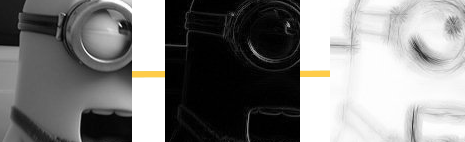
\includegraphics[width=0.4\textwidth]{images/sketch-steps.png}
  \caption{The intermediate results when calculating the line sketches. Left:
  input image, Center: Gradient image, Right: result $L$.}
  \label{fig:sketch-steps}
\end{figure}

\subsection{Shading}
The other important step in creating a believable pencil sketch image from a
natural image, is to produce a hatching texture to create the shading. This is
done in two steps: First the histogram of the input image $I_g$ is matched to a
histogram model that was derived in \cite{mainPaper}. This way the tone
distribution is forced to correspond to tone distributions that were measured in
real pencil sketch images. Then the image of a given hatching pattern is used to
render the hatching texture for the input image. 

\paragraph{Histogram Matching}
Tones in natural images do not follow any specific pattern. In pencil drawings
however, the tones are basically created only from two basic tones, namely the
white paper and the graphite strokes in different strengths. Heavy strokes are
used in very dark areas, mid tone strokes are used to produce impression of 3D
layered information and in bright areas the paper is just left white.
\autoref{fig:real-histograms} shows the tone distributions of some real pencil
sketches. One can easily see the three regions, the peak in the dark regions,
which represent the heavy strokes, the constant distribution in the mid tones,
which are used for the layering and very much bright pixels, originating from
the white paper, that was just left blank.

\begin{figure}[htb]
  \centering
  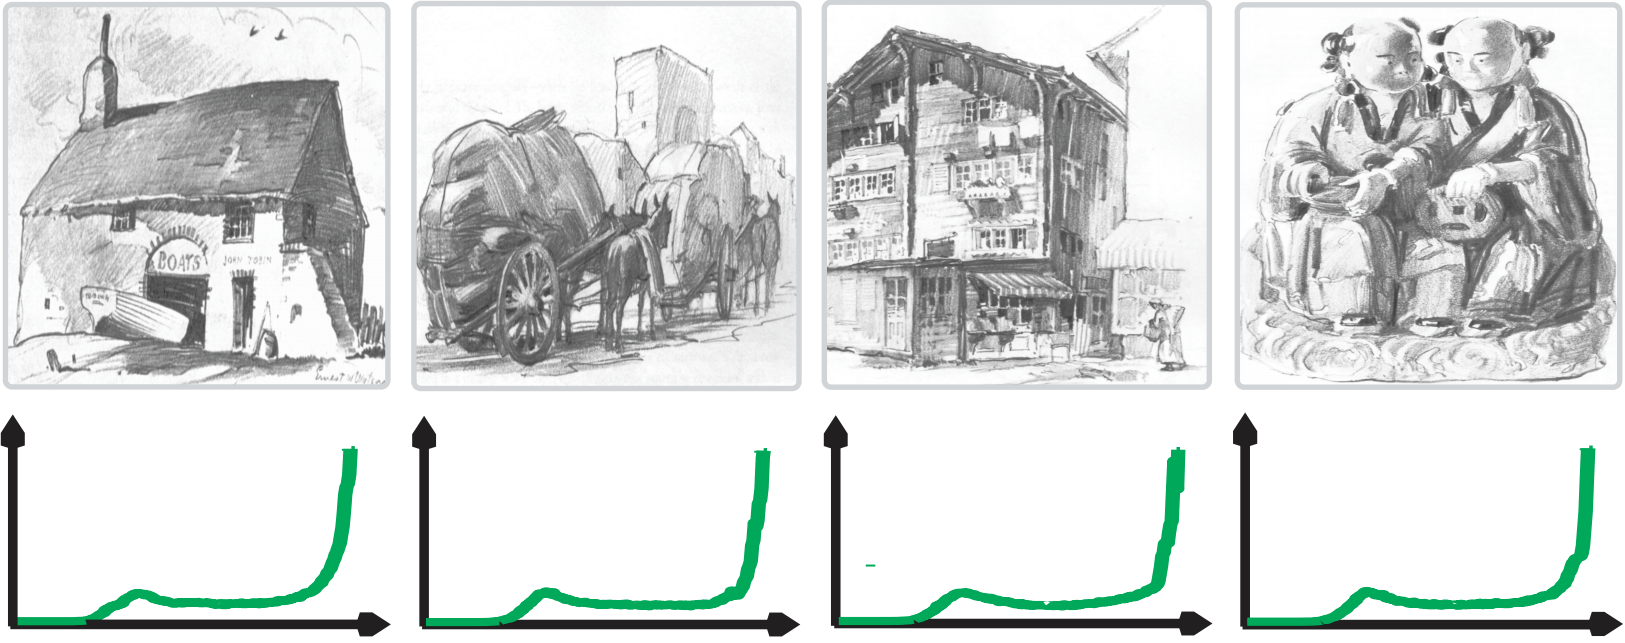
\includegraphics[width=0.4\textwidth]{images/real-histograms.png}
  \caption{Examples for real pencil sketches and their measured tone
    distributions. Note: This image was taken from \cite{mainPaper}}
  \label{fig:real-histograms}
\end{figure}

\cite{mainPaper} used this observation to create a parametric histogram model
for pencil drawings which consists of three functions representing those
three tone levels:

For the bright part of the histogram they use a Laplacian distribution with a
peak at the brightest value. This adds some variation in the bright areas, which
originate from slight illumination variances or the use of a eraser.

\begin{align}
  p_1(v) = \frac{255}{\sigma_b} e ^{-\frac{255-v}{\sigma_b}} \label{eq:p_1}
\end{align}

The parameter for this function is just $\sigma_b$, which controls the sharpness of
the function. This distribution can be seen on the left 
in \autoref{fig:p}.

The mid layer is composed of strokes with different pressures and therefore in
different gray levels. So the distributions of those gray levels is equally
distributed as indicated in the histograms in \autoref{fig:real-histograms}. To
represent this part a constant function was chosen to use all those possible
gray levels.

\begin{align}
  p_2(v) = \begin{cases} \frac{1}{u_b - u_a} & \text{if } u_d < v \leq u_b\\
    0 & \text{otherwise}
  \end{cases} \label{eq:p_2}
\end{align}

The controlling parameters for this function are the range boundaries $u_d$
and $u_b$.

Finally the dark region,which shows up as bell shaped peak in the lower
regions in \autoref{fig:real-histograms},is represented as a Gauss-curve. The
position and shape of the dark regions depend on the maximum pressure an artist is using,
and the softness of the pencil that is used.

\begin{align}
  p_1(g) = \frac{1}{\sqrt{2\pi \sigma_d}} e^{-\frac{(v-\mu_d)^2}{2\sigma_d^2}} 
  \label{eq:p_3}
\end{align}

The width of the bell is controlled with the parameter $\sigma_d$ and the
position with $\mu_d$.

Plots for the three functions can be seen in \autoref{fig:p}.

\begin{figure}[htb]
  \centering
  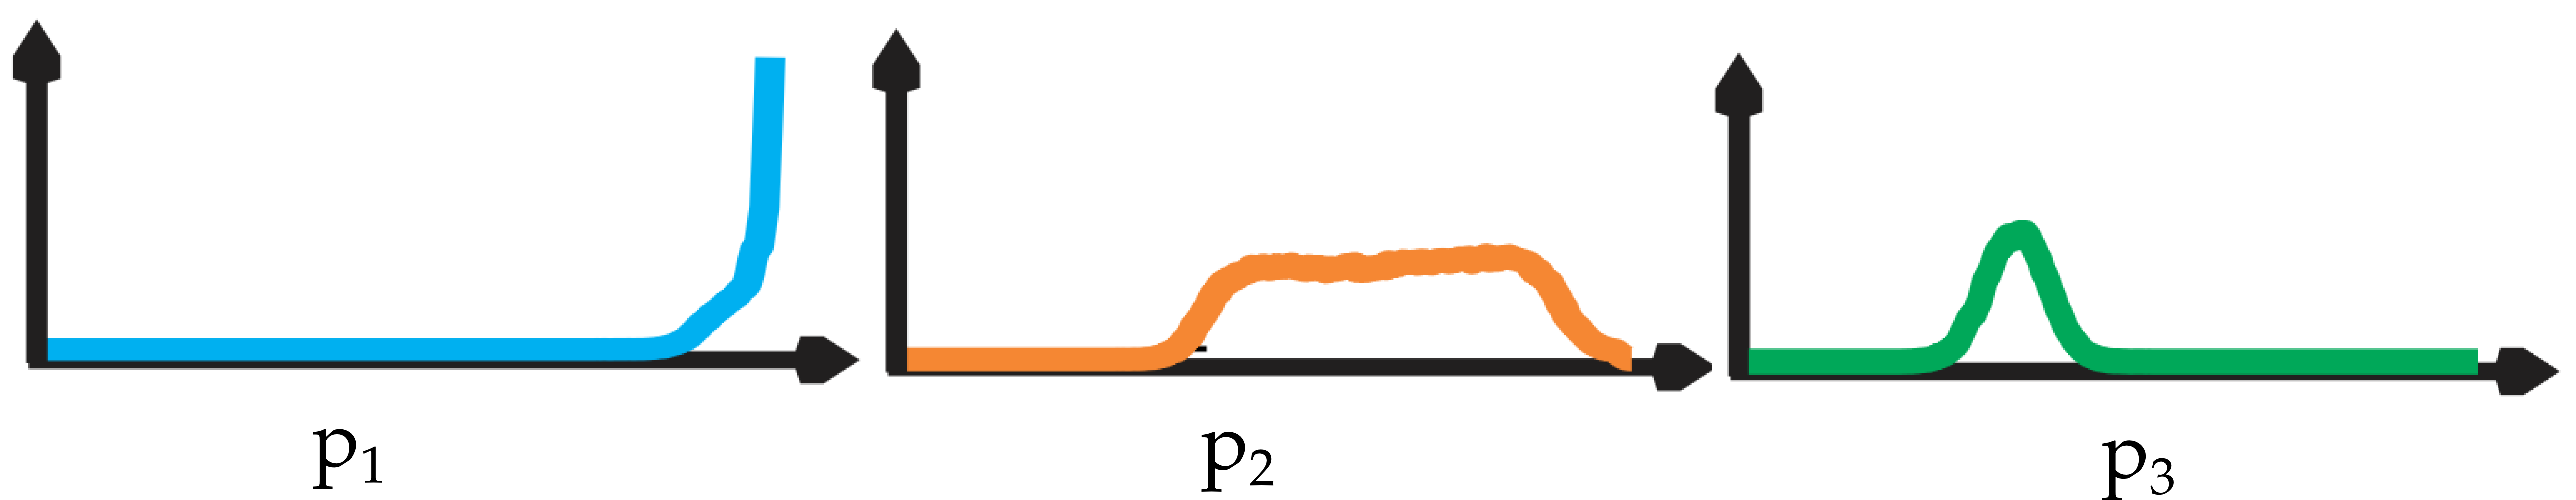
\includegraphics[width=0.4\textwidth]{images/p_i.png}
  \caption{Plots of the three functions $p_i$. Note: picture taken from
    \cite{mainPaper}.}
  \label{fig:p}
\end{figure}

The final tone distribution is now simply composed out of those three
function by creating a weighted sum from $p_1$, $p_2$ and $p_3$:
\begin{align}
  p(v) = \frac{1}{Z} \sum_{i=1}^{3}\omega_i p_i(v)
  \label{eq:p}
\end{align}
Where $Z$ is a normalization factor to make $\int_0^{255}p(v)dv = 1$ and the
$\omega_i$ are weighting parameters which can be used to weight the importance of
the individual Histogram parts.

In \cite{mainPaper} they learned the parameters for those functions from a set
of different styled pencil sketches using Maximum Likelihood Estimation. We skipped this part and left those
parameters to be controlled by the user.

Histogram Matching is then  used to apply the tone distribution from \autoref{eq:p} to
the input image. The result $J$ of the Histogram Matching is then used as input
for the calculation of the hatching texture.  $J$ can be seen on the right side
of \autoref{fig:hist-result}.

\begin{figure}[htb]
  \centering
  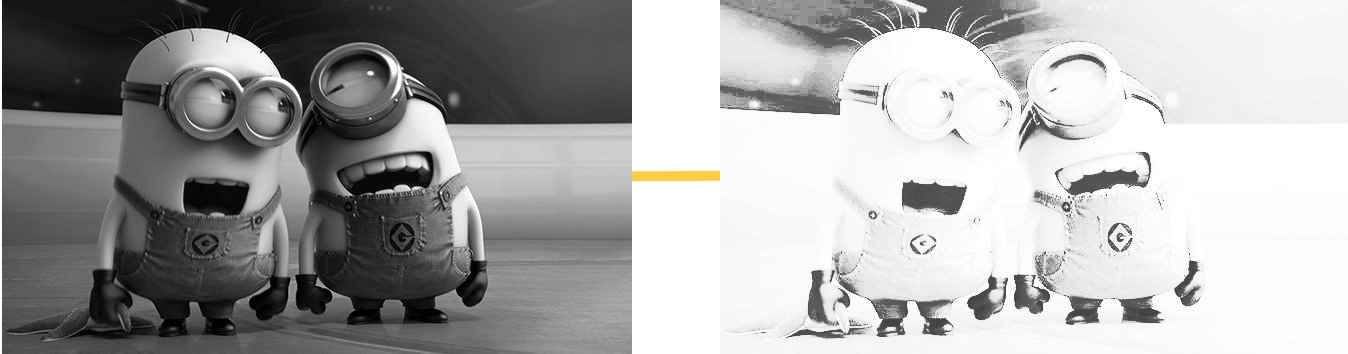
\includegraphics[width=0.5\textwidth]{images/tone-result.png}
  \caption{Left input. Right: Result of Histogram matching for minions.}
  \label{fig:hist-result}
\end{figure}

\paragraph{Texturing}
\begin{figure}[htb]
  \centering
  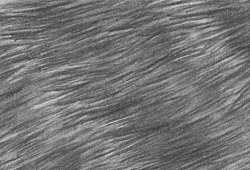
\includegraphics[width=0.4\textwidth]{images/texture2.jpg}
  \caption{A possible men made pencil hatching pattern $H$.}
  \label{fig:hatching-pattern}
\end{figure}
The filter uses a men made pencil hatching pattern $H$ as shown in
\autoref{fig:hatching-pattern}. To create the correct shading in a pencil
sketch, humans repetitively draw on the same position. A exponential function
can be used to simulate this process of placing multiple strokes at the same
position: $H(x)^{\beta(x)} \approx J(x)$. This corresponds to drawing $H$
$\beta$ times at the same position to approximately match the tone that is
dictated by our tonal map $J$. In the logarithmic domain this boils down to
$\beta(x) \ln\left( H(x) \right) \approx \ln\left( J(x) \right)$.



Just solving this equation for $\beta$ is going to destroy the hatching
pattern because $\beta$ can be calculated for each pixel independently, such
that in the end $H^{\beta} = J$. Therefore a smoothness constraint is
introduced:
\begin{align}
  \beta = \arg \min_{\beta}\norm{\beta\ln(H) - \ln(J)}_2^2 + \lambda
  \norm{\nabla \beta}_2^2
  \label{eq:beta}
\end{align}
The smoothness weighting factor $\lambda$ can be used to determine how strong
the hatching pattern $H$ will show through in the resulting image.

The hatching texture $T$ is then calculated as pixelwise exponentiation
\begin{align*}
  T = H^{\beta}
\end{align*}
\autoref{fig:texture-result} shows the result for the minion picture.

\begin{figure}[htb]
  \centering
  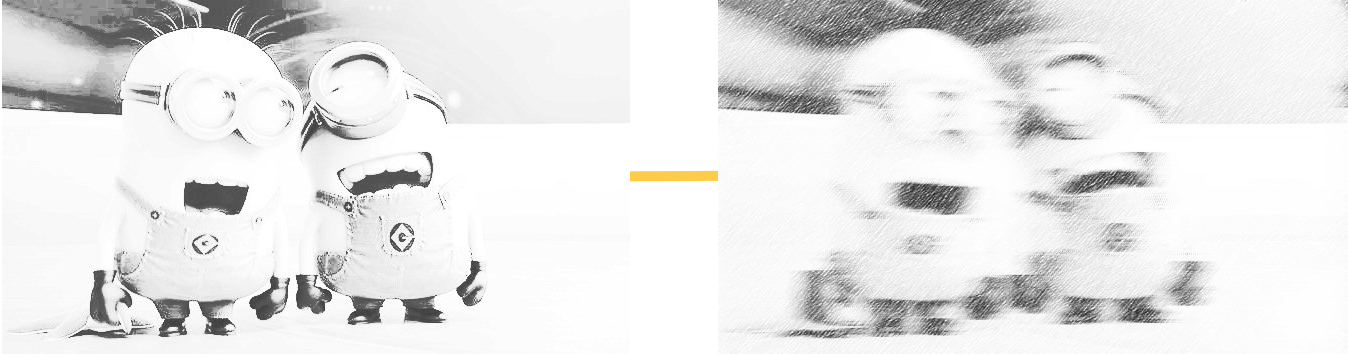
\includegraphics[width=0.5\textwidth]{images/texture-result.png}
  \caption{Left: $J$. Right: Result of texture rendering $T$.}
  \label{fig:texture-result}
\end{figure}



\paragraph{Combining Results}
Finally the results from the line sketching $L$ and the hatching texture $T$ is
combined to the finished pencil drawing $R$ by simply multiplying the images
pixelwise:
\begin{align*}
  R = L  \cdot T
\end{align*}

If desired it is also possible to create colored pencil drawings using the $YUV$
decomposed image $I_{yuv}$ from the beginning and replace the $Y$ channel with
$R$. The resulting RGB-image can then easily be calculated with another color
space transformation.

In \autoref{fig:final-result} both the grayscale and the colored results are shown.

\begin{figure}[htb]
  \centering
  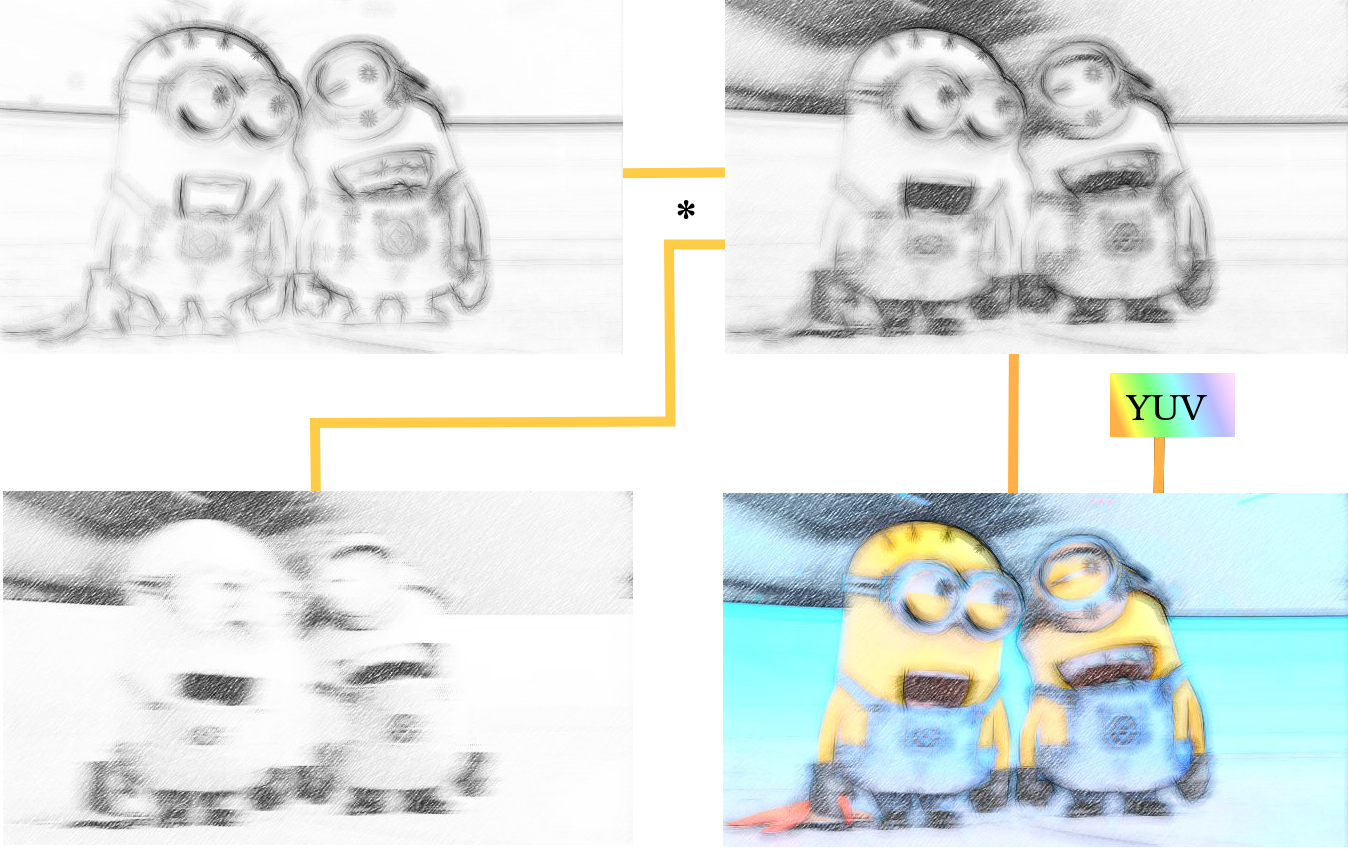
\includegraphics[width=0.5\textwidth]{images/final-result.png}
  \caption{Combination of the line drawing and shading.}
  \label{fig:final-result}
\end{figure}
